\documentclass[10pt,a4paper]{article}
\usepackage[utf8]{inputenc}
\usepackage[english]{babel}
%\usepackage{minted}
\usepackage{listings}
\usepackage{xcolor}
\usepackage{graphicx}

%For syntax highlighting
\definecolor{codegreen}{rgb}{0,0.6,0}
\definecolor{codegray}{rgb}{0.5,0.5,0.5}
\definecolor{codepurple}{rgb}{0.58,0,0.82}
\definecolor{backcolour}{rgb}{1,1,1}

%%Sets different parameters
\lstdefinestyle{mystyle}{
	backgroundcolor=\color{backcolour},   
    commentstyle=\color{codegreen},
    keywordstyle=\color{magenta},
    numberstyle=\tiny\color{codegray},
    stringstyle=\color{codepurple},
    basicstyle=\ttfamily\footnotesize,
    breakatwhitespace=false,         
    breaklines=true,                 
    captionpos=b,                    
    keepspaces=true,                 
    numbers=left,                    
    numbersep=5pt,                  
    showspaces=false,                
    showstringspaces=false,
    showtabs=false,                  
    tabsize=4
}
\lstset{style=mystyle}

\title{\bf Floating Point Operations}
\author{\vspace{-10ex}}
\date{\vspace{-10ex}}
\begin{document}
\maketitle

\begin{minipage}{0.45\textwidth}
        \begin{tabular}{l l}
            \textbf{Expt No:}&9\\
            \textbf{Date :}&16/10/2020
        \end{tabular}
\end{minipage}%
\begin{minipage}{0.45\textwidth}
        \begin{tabular}{l l}
             \textbf{Name:}& Shivanirudh S G  \\
             \textbf{Reg No:} & 185001146 
        \end{tabular}
\end{minipage}
\vspace{1cm}
\hrule

\begin{flushleft}
\subsection*{\textbf{Aim:}} 
To perform floating point operations in 8086.

\vspace{1cm}
\hrule
\subsection*{\textbf{\underline{Floating point Addition}}}

\subsubsection*{\textbf{Algorithm:}}
\begin{itemize}
    \item Move the data segment to the AX register and then move it to the DS register.
    \item Initialise 8087 microprocessor using command FINIT.
    \item Load num1 and num2 onto the 8087 stack using FLD num1 and FLD num2 commands.
    \item Add stack elements 0 and 1 using FADD ST(0), ST(1).
    \item Store the result in sum using FST sum.
\end{itemize}

\newpage
\subsubsection*{\textbf{Program:}}

\begin{table}[htb]
\centering
\resizebox{\columnwidth}{!}{
\begin{tabular}{|l|l|} 
\hline
\textbf{Program}                                                 & \textbf{Comments}                             \\ 
\hline
\hline
assume cs:code, ds:data                                          & Declare code and data segments                \\
\hline
data segment                                                     & Start of data segment                         \\
\hline
org 00H                                                          & Store at offset 00                            \\
\hline
num1 dd 20.4325                                                  & Define decimal word num1 with value 20.4325   \\
\hline
org 10H                                                          & Store at offset 10                            \\
\hline
num2 dd 20.4575                                                  & Define decimal word num2 with value 20.4575   \\
\hline
org 20H                                                          & Store at offset 20                            \\
\hline
sum dd ?                                                         & Define decimal word sum to store result       \\
\hline
data ends                                                        & End of data segment                           \\
\hline
code segment                                                     & Start of code segment                         \\
\hline
start:~mov ax, data                                              & Move data to AX register                      \\
\hline
mov ds, ax                                                       & Move contents of AX register to DS register   \\
\hline
finit                                                            & Initialise 8087 microprocessor                \\
\hline
fld num1                                                         & Load num1 into stack of 8087                  \\
\hline
fld num2                                                         & Load num2 into stack of 8087                  \\
\hline
fadd st(0), st(1)                                                & ST(0) = ST(0) + ST(1)                         \\
\hline
fst sum                                                          & Store value fo ST(0) in sum                   \\
\hline
mov ah, 4ch                                                      & To request interrupt                          \\
\hline
int 21h                                                          & Request interrupt routine                     \\ 
\hline
code ends                                                        & End of code segment                           \\
\hline
end start                                                        &                                               \\
\hline
\end{tabular}
}
\end{table}

\newpage
\subsection*{\textbf{Unassembled code:}}
\begin{figure}[h]
    \centering
    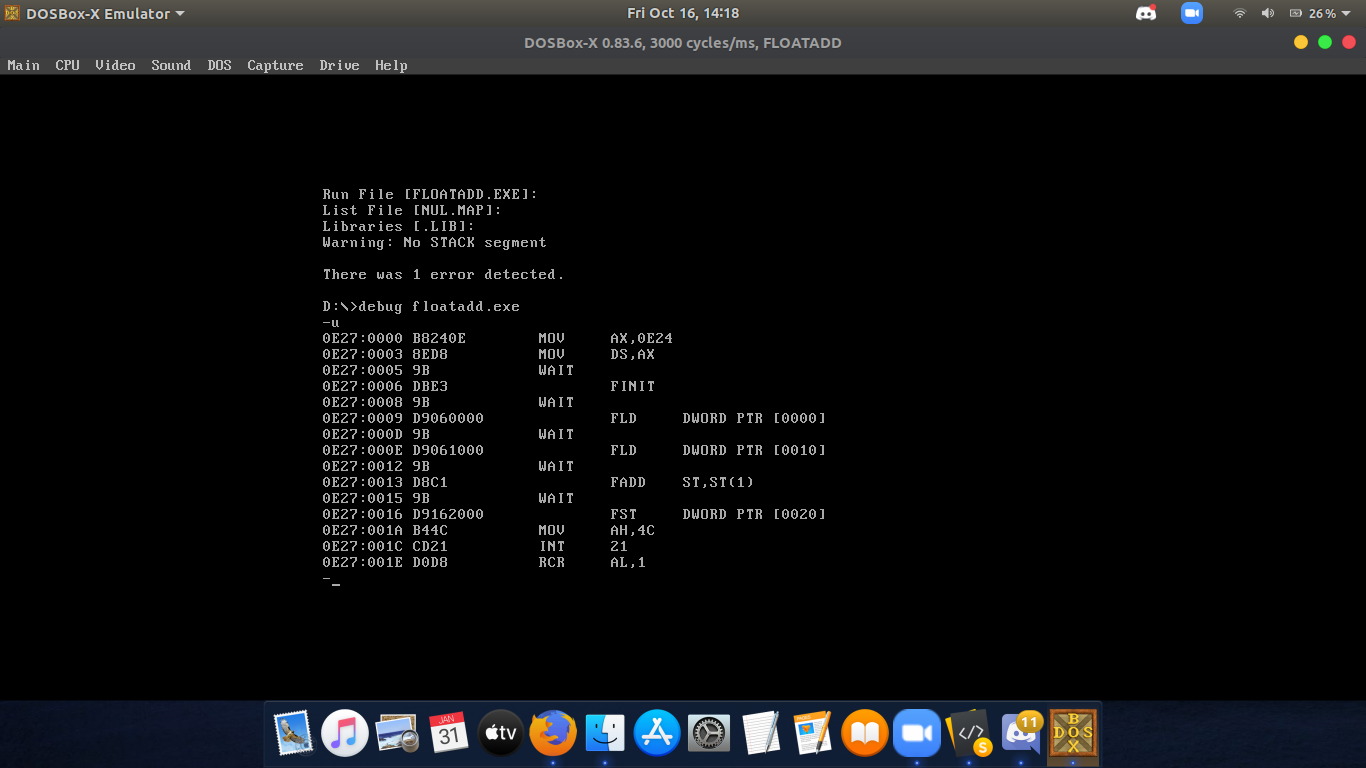
\includegraphics[trim = 100mm 60mm 200mm 110mm, clip, width = \textwidth]{Pics/FAUS.png}
\end{figure}
\subsubsection*{\textbf{Input and Output:}}
\begin{figure}[h]
    \centering
    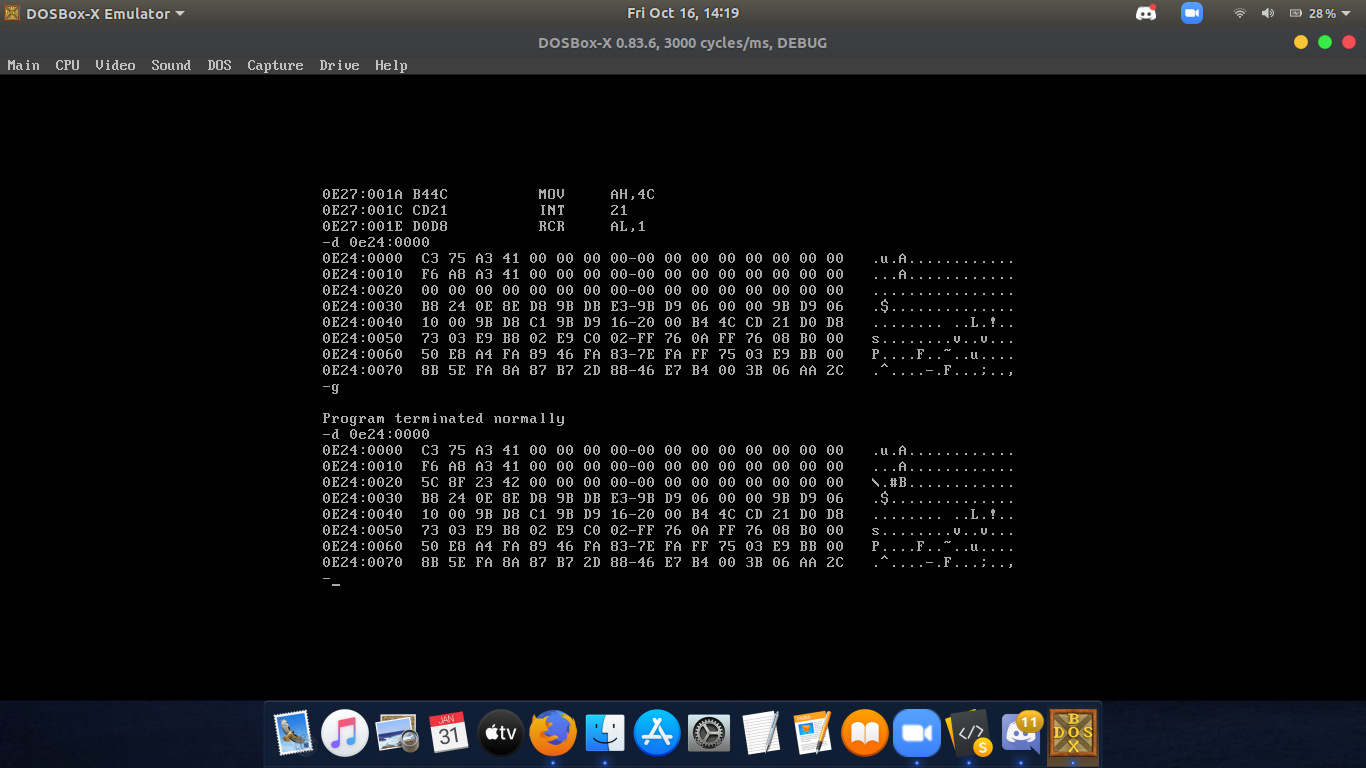
\includegraphics[trim = 100mm 60mm 100mm 80mm, clip, width = \textwidth]{Pics/FAIO.png}
    \caption{ \textbf{Input:} num1: 20.4325, num2: 20.4575; \newline \hspace{1cm}
              \textbf{Output:} sum: 40.69}
\end{figure}
%-------------------------------------------------------------------------------------------------------------------------------------------
\hrule
\newpage
\subsection*{\textbf{\underline{Floating point Addition}}}

\subsubsection*{\textbf{Algorithm:}}
\begin{itemize}
    \item Move the data segment to the AX register and then move it to the DS register.
    \item Initialise 8087 microprocessor using command FINIT.
    \item Load num1 and num2 onto the 8087 stack using FLD num1 and FLD num2 commands.
    \item Add stack elements 0 and 1 using FADD ST(0), ST(1).
    \item Store the result in diff using FST diff.
\end{itemize}

\newpage
\subsubsection*{\textbf{Program:}}

\begin{table}[htb]
\centering
\resizebox{\columnwidth}{!}{
\begin{tabular}{|l|l|} 
\hline
\textbf{Program}                                                 & \textbf{Comments}                             \\ 
\hline
\hline
assume cs:code, ds:data                                          & Declare code and data segments                \\
\hline
data segment                                                     & Start of data segment                         \\
\hline
org 00H                                                          & Store at offset 00                            \\
\hline
num1 dd 20.4325                                                  & Define decimal word num1 with value 20.4575   \\
\hline
org 10H                                                          & Store at offset 10                            \\
\hline
num2 dd 20.4575                                                  & Define decimal word num2 with value 20.4325   \\
\hline
org 20H                                                          & Store at offset 20                            \\
\hline
diff dd ?                                                        & Define decimal word diff to store result      \\
\hline
data ends                                                        & End of data segment                           \\
\hline
code segment                                                     & Start of code segment                         \\
\hline
start:~mov ax, data                                              & Move data to AX register                      \\
\hline
mov ds, ax                                                       & Move contents of AX register to DS register   \\
\hline
finit                                                            & Initialise 8087 microprocessor                \\
\hline
fld num1                                                         & Load num1 into stack of 8087                  \\
\hline
fld num2                                                         & Load num2 into stack of 8087                  \\
\hline
fsub st(0), st(1)                                                & ST(0) = ST(0) + ST(1)                         \\
\hline
fst diff                                                         & Store value fo ST(0) in diff                  \\
\hline
mov ah, 4ch                                                      & To request interrupt                          \\
\hline
int 21h                                                          & Request interrupt routine                     \\ 
\hline
code ends                                                        & End of code segment                           \\
\hline
end start                                                        &                                               \\
\hline
\end{tabular}
}
\end{table}

\newpage
\subsection*{\textbf{Unassembled code:}}
\begin{figure}[h]
    \centering
    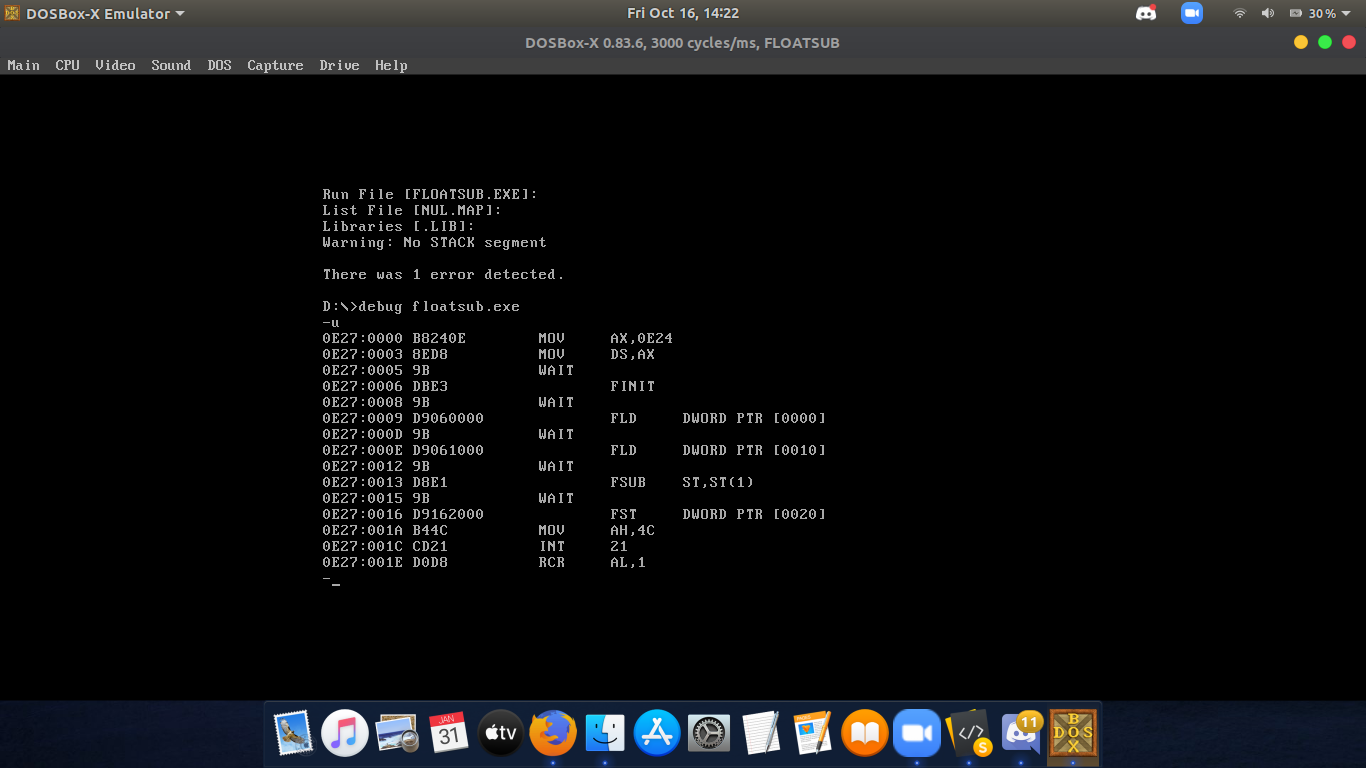
\includegraphics[trim = 100mm 60mm 200mm 110mm, clip, width = \textwidth]{Pics/FSUS.png}
\end{figure}
\subsubsection*{\textbf{Input and Output:}}
\begin{figure}[h]
    \centering
    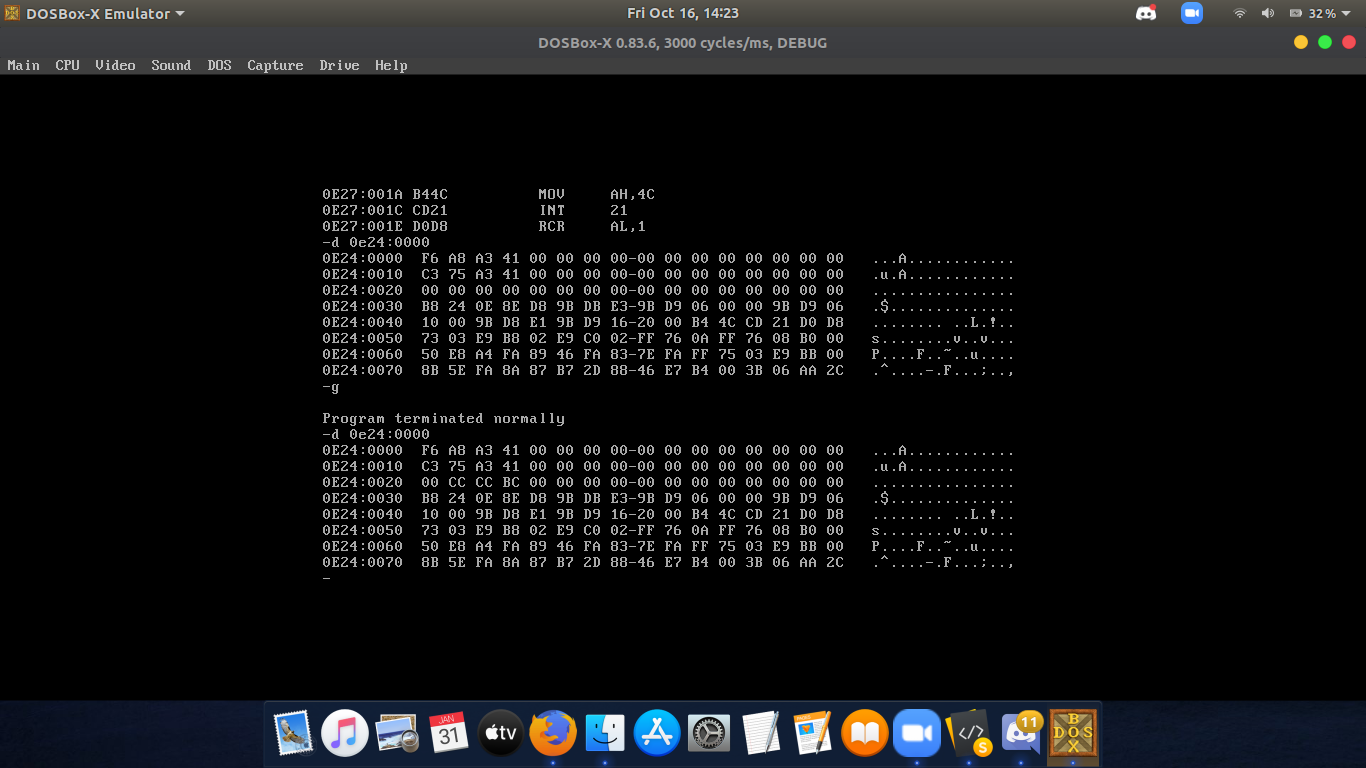
\includegraphics[trim = 100mm 60mm 100mm 80mm, clip, width = \textwidth]{Pics/FSIO.png}
    \caption{ \textbf{Input:} num1: 20.4575, num2: 20.4325; \newline \hspace{1cm}
              \textbf{Output:} difference: 0.025}
\end{figure}
\hrule
\subsection*{\textbf{Result:}}
The 8086 programs were written to perform Floating Point operations, and the results observed.
\end{flushleft}
\end{document}